\documentclass[avery5371, grid,frame]{flashcards}

\usepackage{graphicx}
\usepackage{geometry}

\geometry{a4paper, landscape, margin=0.2in}
\cardfrontstyle[\large\slshape]{headings}
\cardbackstyle{empty}

\begin{document}

\renewcommand{\cardpaper}{a4paper}
\renewcommand{\cardpapermode}{landscape}
\renewcommand{\cardrows}{2}
\renewcommand{\cardcolumns}{2}
\setlength{\cardheight}{3.5in}
\setlength{\cardwidth}{5.0in}
\setlength{\topoffset}{0.50in}
\setlength{\oddoffset}{0.50in}
\setlength{\evenoffset}{0.50in}

\begin{flashcard}{sleep}
    \vspace*{\fill}
    \begin{center}
        \begin{minipage}[c]{.45\textwidth}
            
\includegraphics[width=\textwidth]{cards/s/sleep/sleep - an owl perched on a tree branch, head tucked under its wing, snoozing during the day.png}
        \end{minipage}
        \begin{minipage}[c]{.45\textwidth}
            \begin{itemize}\setlength\itemsep{12pt}
            \item Explanation: \ To rest with your eyes closed and mind and body not active

            \item Example: \ an owl perched on a tree branch, head tucked under its wing, snoozing during the day
            \end{itemize}
        \end{minipage}
    \end{center}
    \vspace*{\fill}
\end{flashcard}\begin{flashcard}{sleep}
    \vspace*{\fill}
    \begin{center}
        \begin{minipage}[c]{.45\textwidth}
            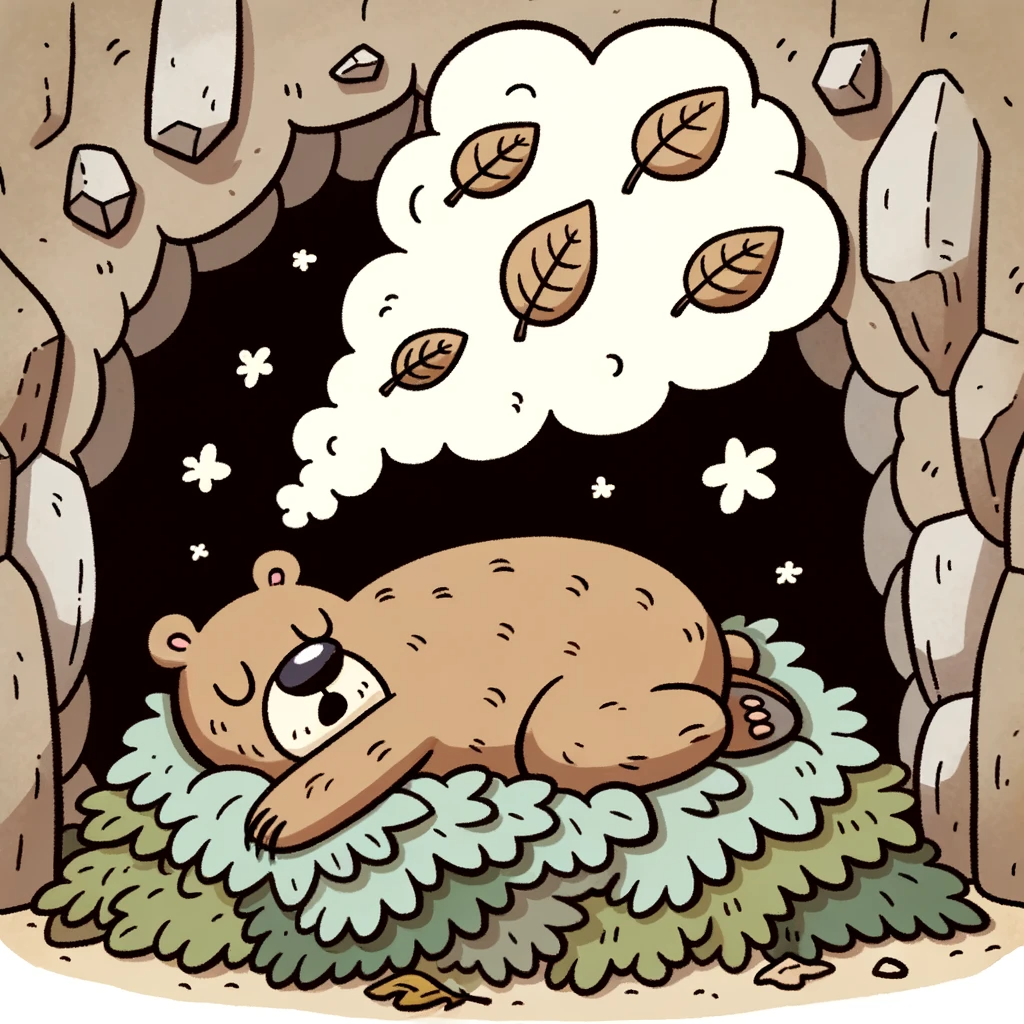
\includegraphics[width=\textwidth]{cards/s/sleep/sleep - a bear hibernating in a cave, surrounded by a pile of leaves, breathing slowly and deeply in slumber.png}
        \end{minipage}
        \begin{minipage}[c]{.45\textwidth}
            \begin{itemize}\setlength\itemsep{12pt}
            \item Explanation: \ To rest with your eyes closed and mind and body not active

            \item Example: \ a bear hibernating in a cave, surrounded by a pile of leaves, breathing slowly and deeply in slumber
            \end{itemize}
        \end{minipage}
    \end{center}
    \vspace*{\fill}
\end{flashcard}\begin{flashcard}{sleep}
    \vspace*{\fill}
    \begin{center}
        \begin{minipage}[c]{.45\textwidth}
            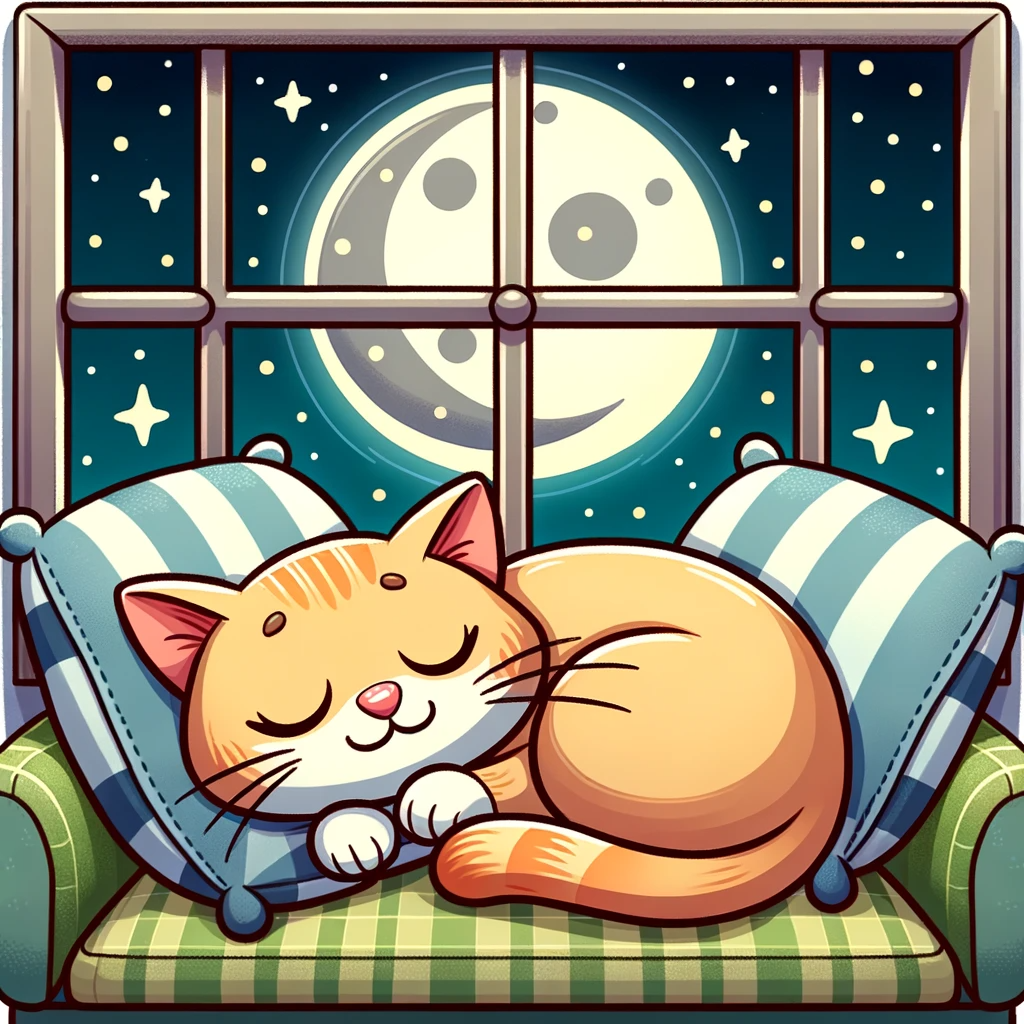
\includegraphics[width=\textwidth]{cards/s/sleep/sleep - a cat curled up, peacefully sleeping on a cushion with a moonlit window in the background.png}
        \end{minipage}
        \begin{minipage}[c]{.45\textwidth}
            \begin{itemize}\setlength\itemsep{12pt}
            \item Explanation: \ To rest with your eyes closed and mind and body not active

            \item Example: \ a cat curled up, peacefully sleeping on a cushion with a moonlit window in the background
            \end{itemize}
        \end{minipage}
    \end{center}
    \vspace*{\fill}
\end{flashcard}\begin{flashcard}{sleep}
    \vspace*{\fill}
    \begin{center}
        \begin{minipage}[c]{.45\textwidth}
            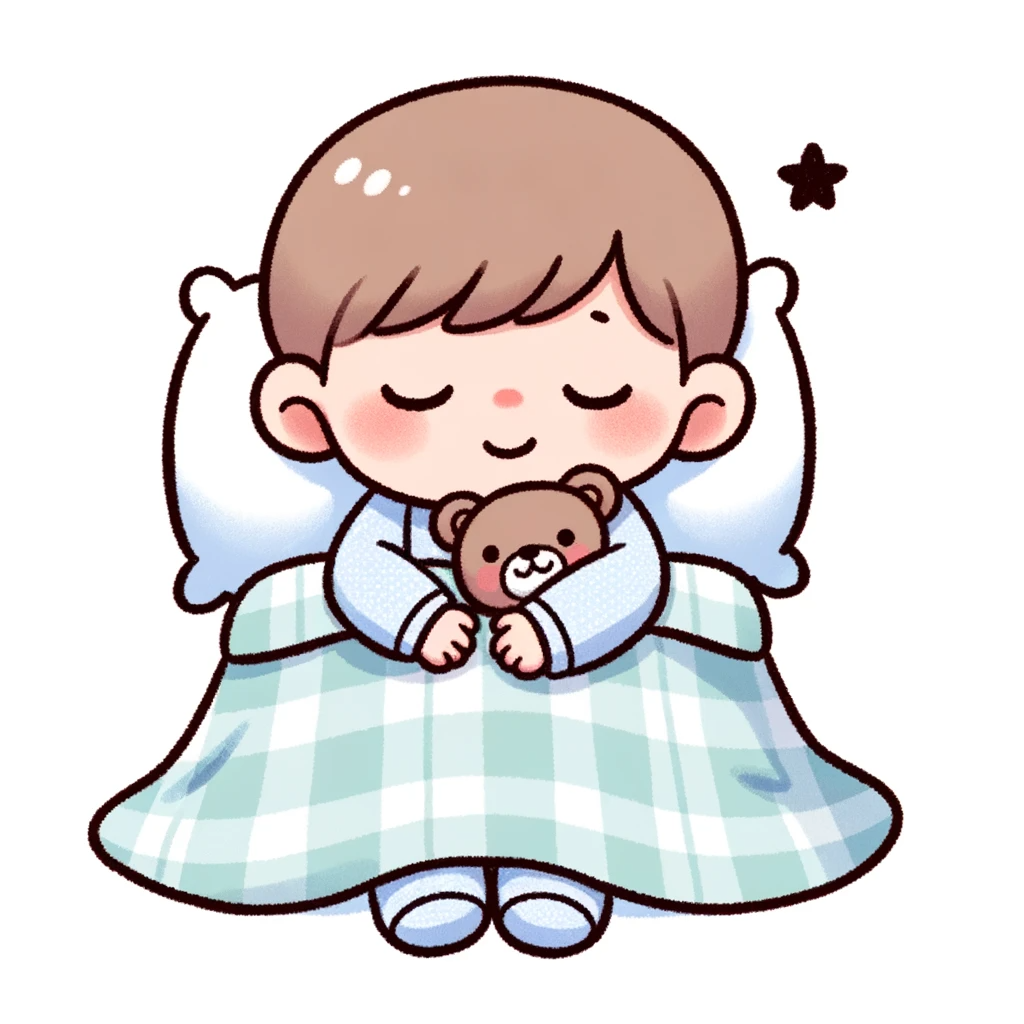
\includegraphics[width=\textwidth]{cards/s/sleep/sleep - a young child in pajamas, snuggled under a blanket with a teddy bear, eyes closed in deep sleep.png}
        \end{minipage}
        \begin{minipage}[c]{.45\textwidth}
            \begin{itemize}\setlength\itemsep{12pt}
            \item Explanation: \ To rest with your eyes closed and mind and body not active

            \item Example: \ a young child in pajamas, snuggled under a blanket with a teddy bear, eyes closed in deep sleep
            \end{itemize}
        \end{minipage}
    \end{center}
    \vspace*{\fill}
\end{flashcard}

\end{document}